\documentclass[./Differential Equations.tex]{subfiles}

\begin{document}
	\section{Solution Curves without a Solution}
		If a DE is not explicitly or analytically solvable, it still provides information regarding its solution curve.
		\subsection{Direction Fields}
			\subsubsectionb{Slope}
				As the solution \(y = y(x)\) of the first order DE
					\[\dv{y}{x} = f(x, y)\]
					must be differentiable on its interval of definition \(I\), it must also be continuous on said interval. The function \(f\) in normal form, as presented above, is called the \textbf{slope/rate function}. The slope of the tangent line at point \((x, y(x)\) is equal to \(f(x, y(x))\). \\
				Let \((x, y)\) represent any point in the \(xy\)-plane for which \(f\) is defined. The value of the function at that point represents the slope of a line segment called a \textbf{lineal element}, which is some segment of the tangent line at that point.
			\subsubsectionb{Direction Field}
				A \textbf{direction/slope field} is a plot of small lineal elements over some region in the \(xy\)-plane. Visually, it provides information regarding the shape of a family of solution curves, allowing qualitative aspects of said family to be discerned. A solution curve passing through the field must follow the flow of the grid, being tangent to the lineal element at any point it intersects one.
			\subsubsectionb{Increasing/Decreasing}
				The sign of the first derivative provides information regarding whether the function is increasing or decreasing.
					\[\begin{tabular}{|c|c|c|}\hline
						\(\dv*{y}{x}\) & \(< 0\) & \(> 0\) \\\hline
						function behavior & decreasing & increasing \\\hline
					\end{tabular}\]
		\subsection{Autonomous First-Order DEs}
			\subsubsectionb{Autonomous First-Order DEs}
				An ODE that does not explicitly contain the independent variable is said to be \textbf{autonomous}. If \(x\) is independent and \(y\) is dependent, an autonomous DE would take the form
					\[f(y, y') = 0 \qquad \text{or} \qquad \dv{y}{x} = f(y)\]
					It is assumed that \(f\) isa  continuous and differentiable function of \(y\) on some interval \(I\).
			\subsubsectionb{Critical Points}
				A real number \(c\) is a \textbf{critical/equilibrium/stationary point} of an autonomous DE if \(f(c) = 0\). If the constant function \(y(x) = c\) is substituted into the normal form of an autonomous de, both sides equate to 0.
				\callout{14.19}{
					\textit{If \(c\) is a critical point of an autonomous DE, then \(y(x) = c\) is a constant solution.}
				}
				A constant solution \(y(x) = c\) is also referred to as an \textbf{equilibrium solution}, equilibria being the \textit{only} constant solutions.
				A \textbf{(one dimensional) phase portrait} consists of a vertical \textbf{phase line} (the \(P\)-axis) displaying the intervals on which a function is increasing or decreasing between equilibria.
			\subsubsectionb{Solution Curves}
				As \(f\) is independent of \(x\), it may be considered defined for \(-\infty < x < \infty\) or \(0 \le x < \infty\). As \(f\) is continuous and differentiable for \(y\) on some interval \(I\) of the \(y\)-axis, some horizontal region \(R\) can be formed in the \(xy\)-plane using \(I\). Through any point \(x_0, y_0\) in \(R\) passes only a single solution curve. \\
				Suppose \(R\) is split into subregions \(R_i\) by equilibria \(y(x) = c_i\). 
				\begin{itemize}
					\item
						If a solution curve passes through point \(x_i, y_i\) in \(R_i\), it must stay within \(R_i\) for all \(x\), as the curve is continuous and cannot cross equilibria.
					\item
						As \(f\) is continuous over \(R\), \(f(y)\) must be either entirely positive or entirely negative for all \(x\) in \(R_i\).
					\item
						As \(\dv*{y}{x} = f(y(x))\), all solution curves must be monotonic.
					\item
						If \(y(x)\) is \textit{bounded} by 1 or 2 critical points, then the graph must asymptotically approach them.
				\end{itemize}
			\subsubsectionb{Attractors and Repellers}
				A critical point \(c\) may be an \textbf{attractor} of \(y(x)\), an initial point sufficiently close resulting in \(\displaystyle\lim_{x\to \infty} y(x) = c\), a \textbf{repeller}, an initial point sufficiently close resulting in movement away from \(c\), or neither, attracting on one side and repelling on the other. Respectively, these are referred to as \textbf{asymptotically stable}, \textbf{unstable}, and \textbf{semi-stable}.
				\[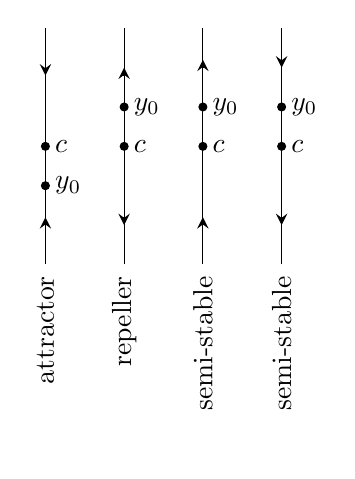
\begin{tikzpicture}
					\node[rotate = 90, align = right, text width = 2.1cm] at (0, -1.2) {attractor};
						\draw[] (0, 0) -- (0, 3);
						\filldraw (0, 1.5) circle (0.5mm) node[right]{\(c\)};
						\filldraw (0, 1) circle (0.5mm) node[right]{\(y_0\)};
						\draw[-stealth, thick] (0, 0.5) -- (0, 0.6);
						\draw[-stealth, thick] (0, 2.5) -- (0, 2.4);
					\node[rotate = 90, align = right, text width = 2.1cm] at (1, -1.2){repeller};
						\draw[] (1, 0) -- (1, 3);
						\filldraw (1, 1.5) circle (0.5mm) node[right]{\(c\)};
						\filldraw (1, 2) circle (0.5mm) node[right]{\(y_0\)};
						\draw[-stealth, thick] (1, 0.6) -- (1, 0.5);
						\draw[-stealth, thick] (1, 2.4) -- (1, 2.5);
					\node[rotate = 90, align = right, text width = 2.1cm] at (2, -1.2){semi-stable};
						\draw[] (2, 0) -- (2, 3);
						\filldraw (2, 1.5) circle (0.5mm) node[right]{\(c\)};
						\filldraw (2, 2) circle (0.5mm) node[right]{\(y_0\)};
						\draw[-stealth, thick] (2, 0.5) -- (2, 0.6);
						\draw[-stealth, thick] (2, 2.5) -- (2, 2.6);
					\node[rotate = 90, align = right, text width = 2.1cm] at (3, -1.2){semi-stable};
						\draw[] (3, 0) -- (3, 3);
						\filldraw (3, 1.5) circle (0.5mm) node[right]{\(c\)};
						\filldraw (3, 2) circle (0.5mm) node[right]{\(y_0\)};
						\draw[-stealth, thick] (3, 0.6) -- (3, 0.5);
						\draw[-stealth, thick] (3, 2.6) -- (3, 2.5);	
				\end{tikzpicture}\]
			\subsubsectionb{Autonomous DEs and Direction Fields}
				As \(\dv*{y}{x}\) is solely dependent on \(y\), the slopes of the lineal elements displayed in a direction field will depend solely on the points' \(y\)-coordinates. \\
				Lineal elements that pass through the same \textit{horizontal} line have the same slopes while those that pass through the same \textit{vertical} line may vary.
			\subsubsectionb{Translation Property}
				\callout{17.4}{
					\textit{If \(y(x)\) is a solution to an autonomous DE, then \(y_1(x) = y(x - k)\) where \(k\) is a constant is as well.}
				}
				This is due to the fact that an autonomous DE is not dependent on \(x\) while the solution curve is.
	\section{Separable Equations}
		The simplest of all DEs fall under the category of first-order separable ODEs.
		\subsectionb{Solution by Integration}
			When \(\dv*{y}{x}\) is solely dependent on \(x\) (\(f(x, y) = g(x)\), integration can be used to solve the DE. If both sides are continuous,
				\[y = \int{g(x)}\dd{x} = G(x) + C\]
		\subsectionb{A Definition}
			\callout{9.56}{\paragraph{Separable Equation}
				A first-order DE of the form
					\[\dv{y}{x} = g(x)h(y)\]
					is said to be \textbf{separable}, having \textbf{separable variables}.
			}
			From this form, it can be seen that
				\[p(y)\dv{y}{x} = g(x)\]
				where \(p(y) = 1/h(y)\). The derivative can then be split so that both differentials are in the numerator.
				\[\int p(y)\dd{y} = \int g(x)\dd{x}\]
				Integrating,
					\[P(y) = G(x) + C\] 
		\subsectionb{Method of Solution}
			A on-parameter family of solutions can be obtained by integrating.\footnote{It should be noted that there is no need for multiple constants of integration for a separable equation, as their difference can simply be replaced by a single constant.}
		\subsectionb{Losing a Solution}
			It should be noted that variable divisors may be zero at a point. Constant solutions are often lost through division.
		\subsectionb{Use of Computers}
			A computer algebra system (CAS) can be used to produce level curves defined by equating the implicit solution \(G(x, y)\) to various values of \(c\). \\
			It should be noted that an IVP may have nontrivial solutions that are part of the same family. In fact, all member of a family may be solutions.
		\subsectionb{An Integral-Defined Function}
			The solution of an IVP \(\dv*{y}{x} = g(x)\), \(y(x_0) = y_0\) defined on interval \(I\) containing \(x_0\) and \(x\) over which \(g\) is continuous is given by
				\[y(x) = y_0 + \int_{x_0}^x g(t)\dd{t}\]
				When the integral is nonelementary, this is acceptable as a final solution.
	\section{Linear Equations}
		\subsectionb{A Definition}
			\callout{12.1}{\paragraph{Definition 2.3.1. Linear Equation}
				A first-order DE of the form
					\[a_1(x)\dv{y}{x} + a_0(x)y = g(x)\]
					is a \textbf{linear equation} in \(y\).
			}
		\subsectionb{Standard Form}
			By dividing by \(a_1(x)\), the \textbf{standard form} of a first-order linear equation is obtained:
				\[\dv{y}{x} + P(x)y = f(x)\]
				A solution of this should be on an interval \(I\) over which both \(P\) and \(f\) are continuous.
		\subsectionb{Method of Solution}
			The left hand side of the standard form of a first-order linear DE can be rewritten as the derivative of a product by multiplying by \(\mu(x)\).
			\[\dv{}{x}[\mu(x)] = \mu\dv{y}{x} + \dv{\mu}{x}y = \mu\dv{y}{x} + \mu Py\]
			Evidently,
			\[
				\dv{\mu}{x} = \mu P \implies 
					\frac{\dd{\mu}}{\mu} = P \dd{x} \implies
					\ln|\mu| = \int P(x)\dd{x} \implies
					\mu = \en^{\int P(x)\dd{x}}
			\]
			The constant of integration is chosen to be 1 for simplicity. This result is called the \textbf{integrating factor}. Substituting in,
			\[
				\dv{}{x}{\Bigl[y\en^{\int P(x)\dd{x}}\Bigr] = \int P(x)\dd{x}}\dv{y}{x} + P(x)\en^{\int P(x)\dd{x}}y = \en^{\int P(x)\dd{x}}f(x)
			\]
			Integrating both sides,
			\[y\en^{\int P(x)\dd{x}} = \int \en^{\int P(x)\dd{x}}f(x)\dd{x}\]
			Solving for \(y\) produces a one-parameter family of solutions
			\[y = \en^{-\int P(x)\dd{x}}\left(\int \en^{\int P(x)\dd{x}}f(x)\dd{x} + C\right)\]
			\callout{17}{\paragraph{Solving a First-Order Linear DE}
				\begin{enumerate}
					\item
						Put the equation into standard form.
					\item
						Identify \(P(x)\) to find the integrating factor \(\en^{\int P(x)\dd{x}}\). Evaluate the integral, forgoing the integration constant.
					\item
						Multiply both sides by the integrating factor:
							\[\dv{y}{x}\Bigl[y\en^{\int P(x)\dd{x}}\Bigr] = \en^{\int P(x)\dd{x}}f(x)\]
					\item
						Integrate both sides and solve for \(y\).
				\end{enumerate}

			}
		\subsectionb{General Solutions}
			Suppose \(P\) and \(f\), found in the standard form of a first-order linear DE, are continuous on \(I\). \textit{If} a solution of the DE exists on \(I\), it must be of the form found via the integrating factor. Conversely, any function in this form is a solution on \(I\). In other words, the family of solutions found via the integrating factor contains \textit{every} solution defined on \(I\).
\end{document}
